\begin{figure}[ptb]
\begin{center}
% \subcaptionbox{The original PIPE 4 tangle graph reporting four tangles of size 18, 10, 7 and 5.}{
%     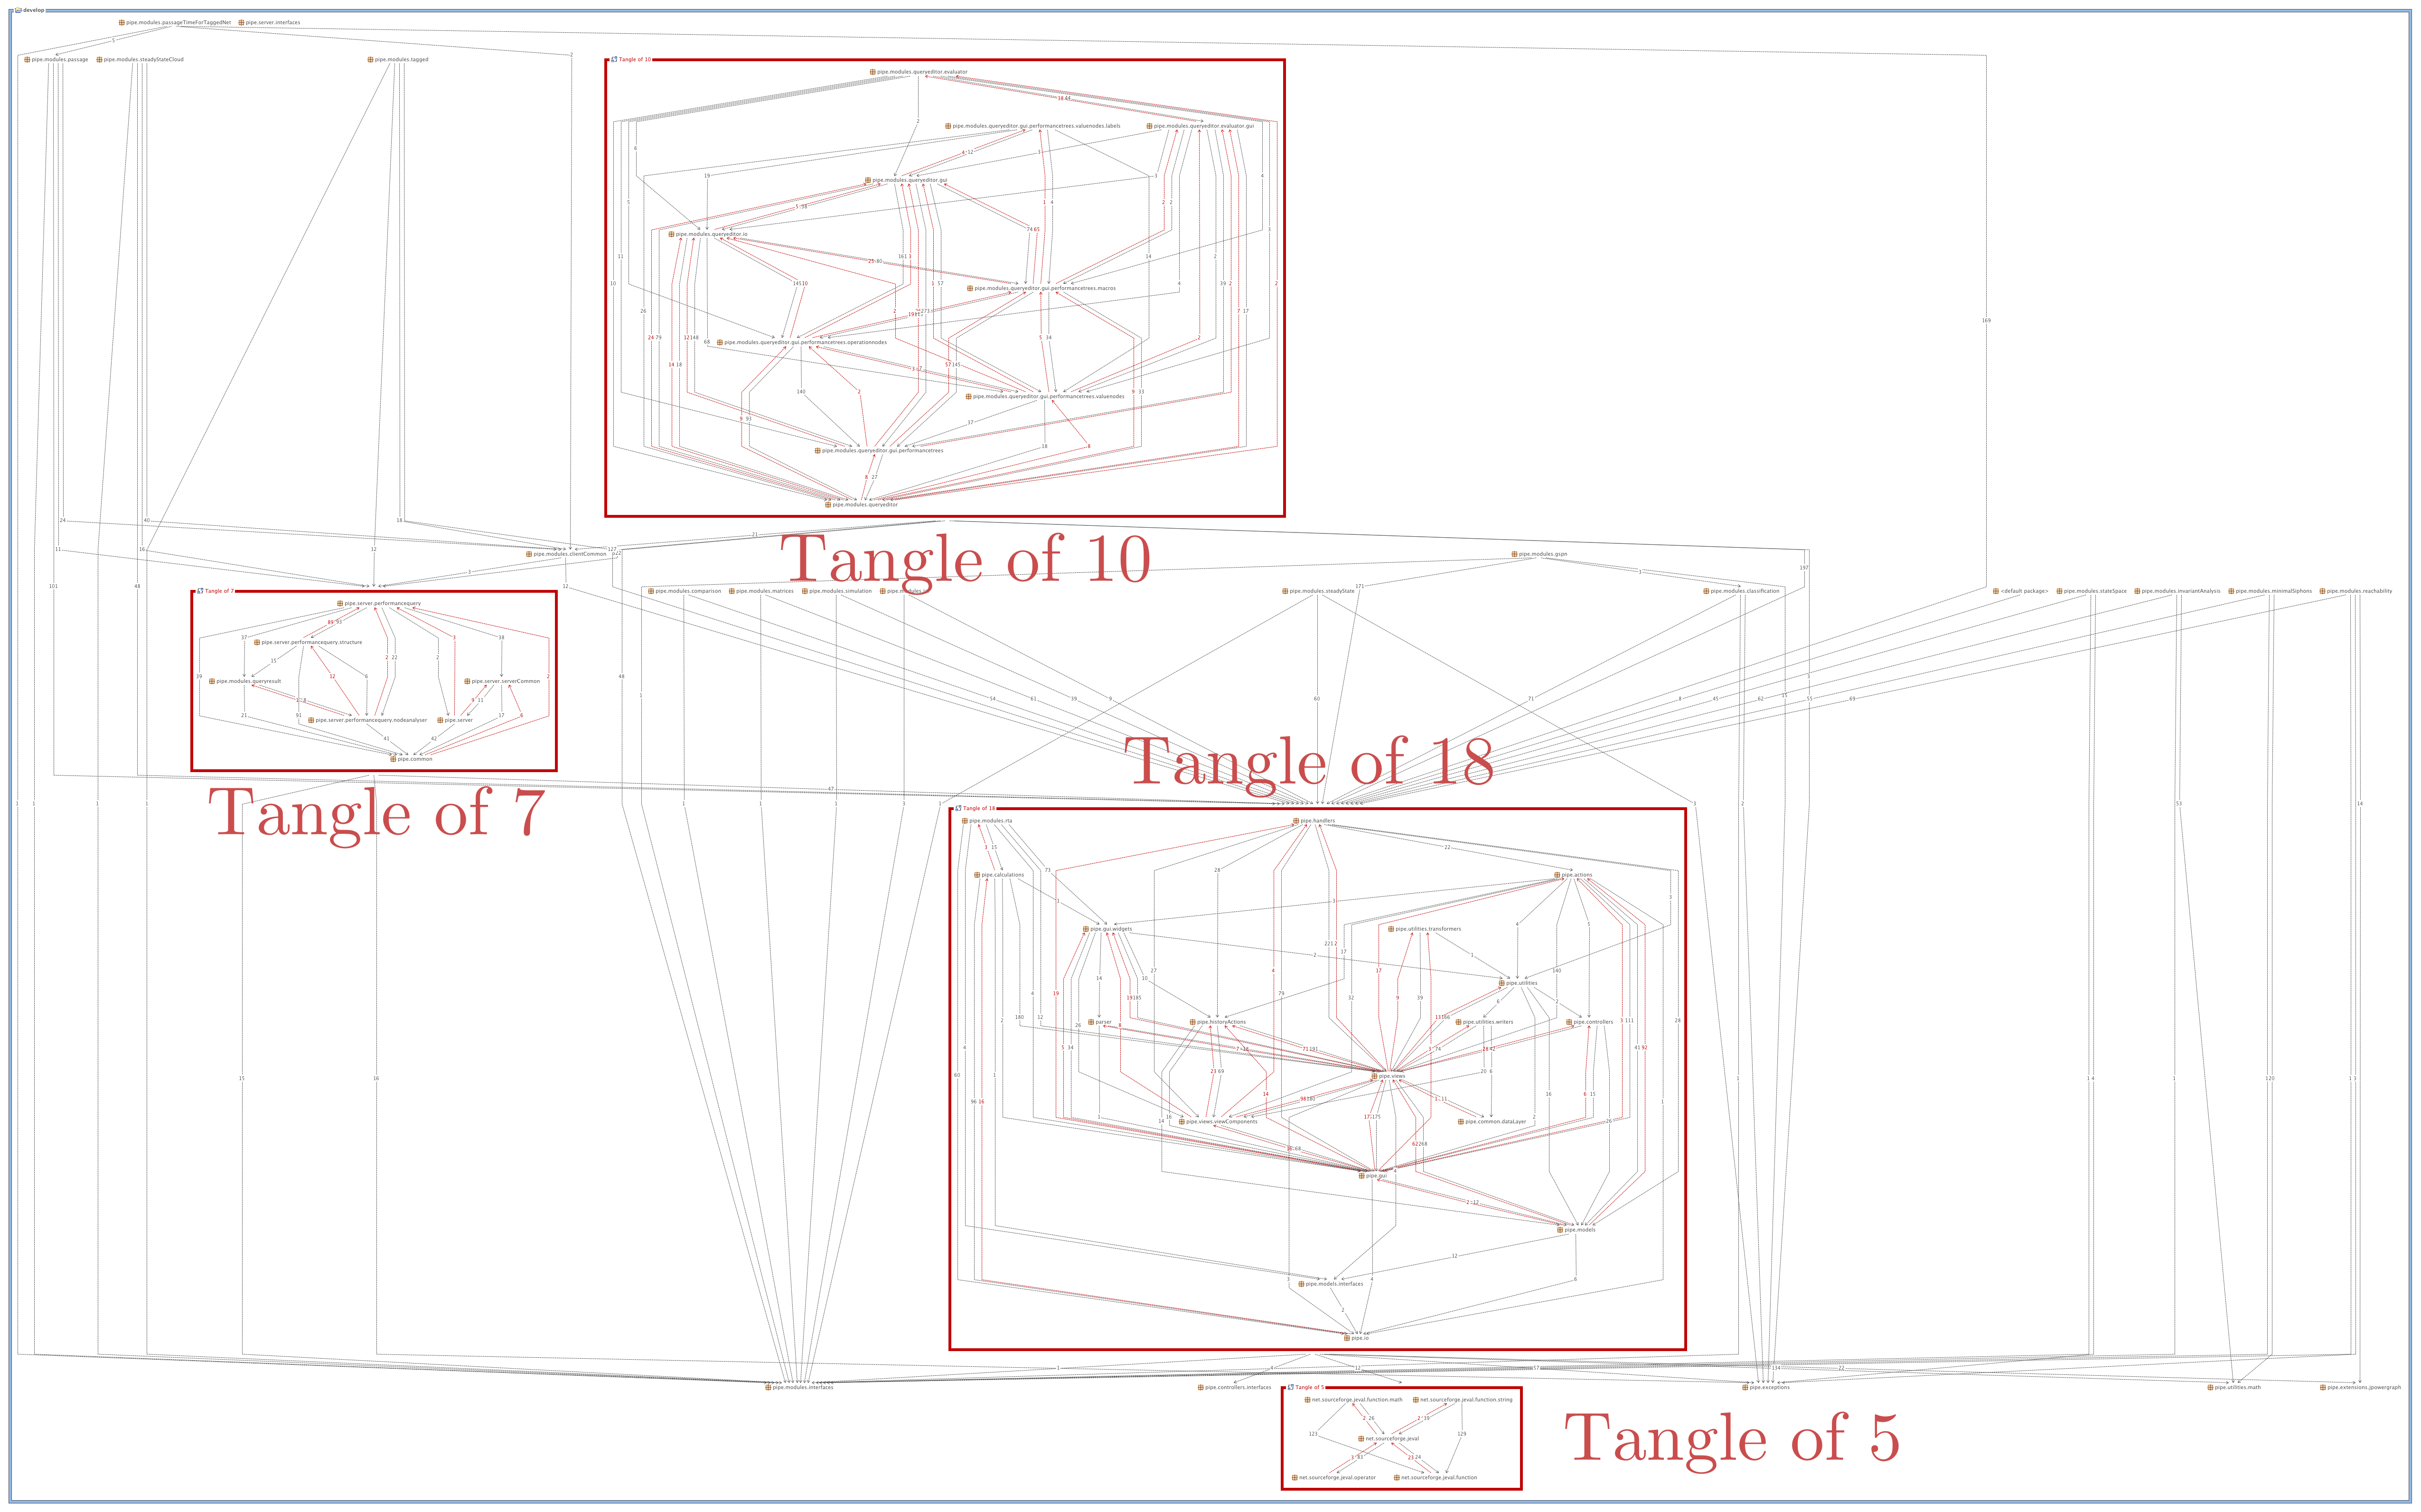
\includegraphics[width=0.85\textwidth]{eval/original_tangle_annotated.png} 
% }
\subcaptionbox{The tangle graph for the PIPE repository housing the view code in PIPE 5 which contains the Swing GUI code. It contains only a single tangle of size 11.}{
    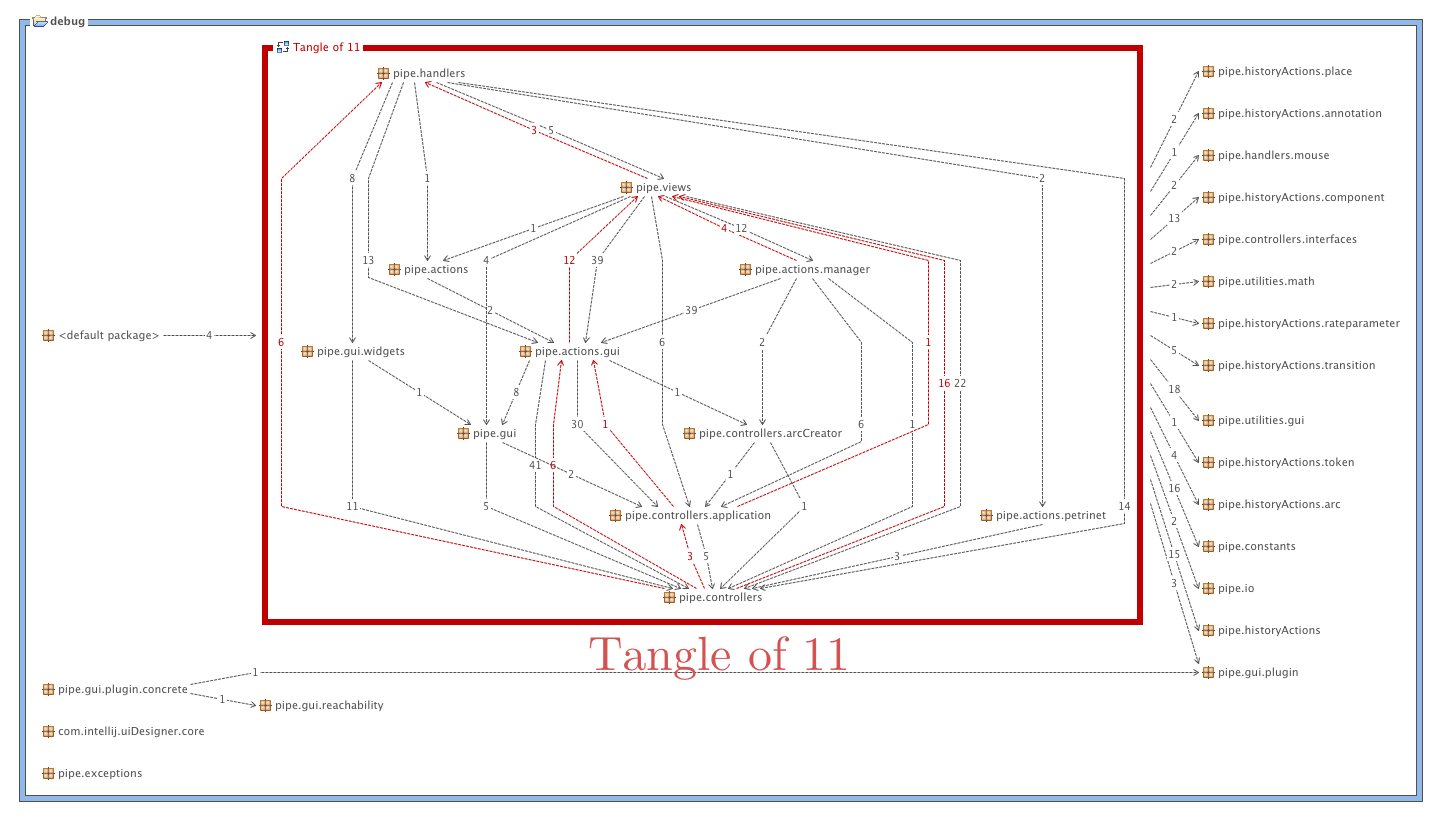
\includegraphics[width=0.85\textwidth]{eval/gui_tangle_annotated.png} 
}

\subcaptionbox{The new PIPE 5 tangle graph for the core repository reporting a single tangle of size 2.}{
    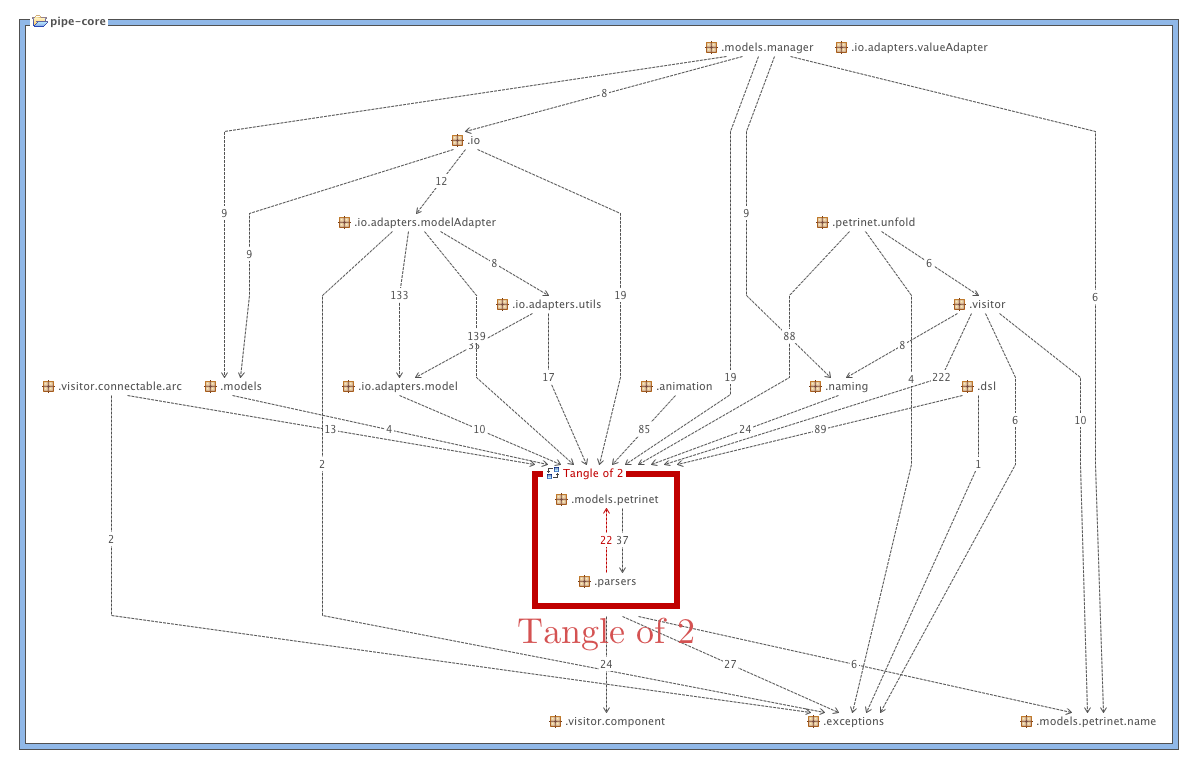
\includegraphics[width=0.85\textwidth]{eval/pipe_core_tangle_annotated.png} 
}
% \subcaptionbox{The tangle graph for the new PIPEAnalysis repository containing the code for the steady state solver and the state space exploration. It reports 0 tangles.}{
%     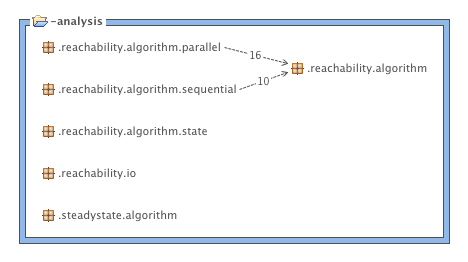
\includegraphics[scale=0.4]{eval/pipe_analysis_tangle.png} 
% }
% \hspace{5mm}
% \subcaptionbox{The tangle graph for the new PIPEMarkovChain repository containing the classes which represent the underlying Markov chain of a Petri net and the explored sets data structure. It reports 0 tangles.}{
%     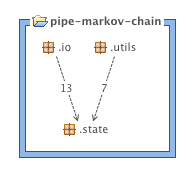
\includegraphics[scale=0.6]{eval/pipe_markov_chain_tangle.png} 
% }
\caption{The tangle graphs for the new PIPE 5 architecture.}
\label{fig:tangle_results}
\end{center}
\end{figure}